\documentclass[../monografia.tex]{subfiles}

\graphicspath{ {images/}{../images/} } % deixei aqui pra parar de aparecer erro, tava me irritando, só comentar de volta

\begin{document}



Para o desenvolvimento do projeto, dividimos as tarefas entre 3 áreas: Hardware, Firmware e Software. 

No \textbf{hardware} estará concentrado todo o desenvolvimento da eletrônica dos dispositivos que estarão nos nós da rede. 
O \textbf{firmware} será todo o software embarcado no dispositivo, desde a comunicação com o hardware até a comunicação sem fio, entre os dispositivos da rede e do dispositivo \textit{gateway} com a plataforma. 
O \textbf{software}, por fim, trata do desenvolvimento relacionado à plataforma onde os dados serão armazenados e apresentados. 

\section{Protótipo}

A partir das especificações técnicas, foi elaborado um novo diagrama de blocos. 

\begin{figure}[h]
    \centering
    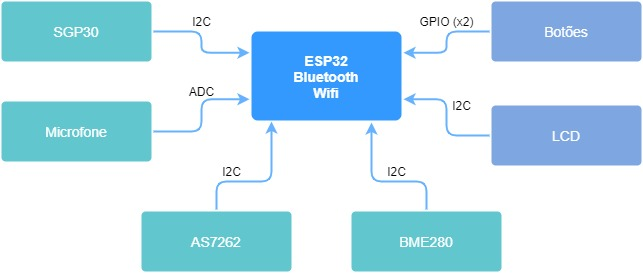
\includegraphics[width=12cm]{diagrama_hw_v1}
    \caption{Diagrama de Blocos de Hardware do Protótipo}
    \label{fig:img1}
\end{figure}

Quando possível, foram utilizados kits de desenvolvimento e módulos que nos permitisse uma validação mais rápida do hardware nessa fase inicial, permitindo avançar mais com o firmware e fazer testes em campo. 

O DevKitC do ESP32 possui integrado um USB, através do qual é possível alimentar os demais subcircuitos da placa, não existindo a necessidade de uso de bateria nessa etapa. 

\subsection{Esquemático}

Para o design do hardware, utilizamos o software de CAD de PCB \textit{Altium Designer 20} \cite{altium}. Foi utilizada a licença da empresa orientadora, sendo possível também conseguir uma licença gratuita para estudantes. Os arquivos estão disponíveis em \cite{git_hw}. 

A partir do diagrama de blocos, foi desenvolvido o esquema elétrico

\begin{figure}[h]
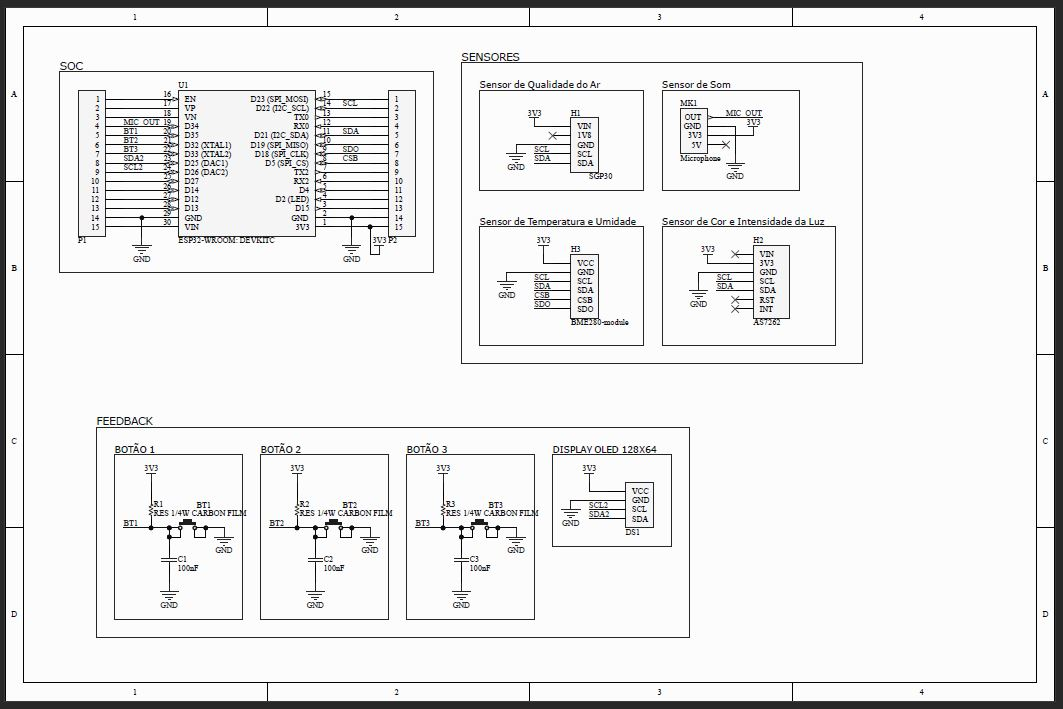
\includegraphics[width=\textwidth]{sch}
\caption{Esquemático do Protótipo}
\label{fig:img2}
\end{figure}

\subsection{PCB - \textit{Printed Circuit Board}}

A placa foi pensada como \textit{Single Layer}, para ser fabricada em fibra por uma fresadora CNC, com seus componentes e conectores soldados à mão. 

\begin{figure}[h!]
\centering
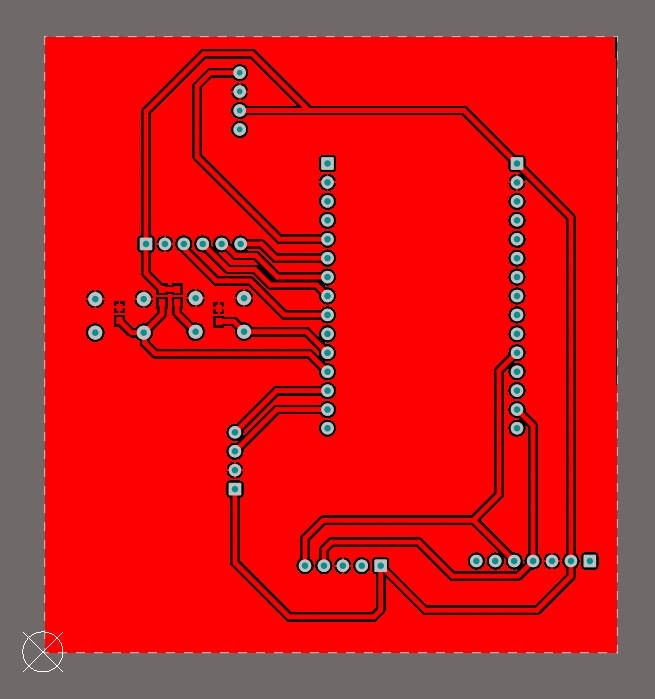
\includegraphics[width=8cm]{pcb_2}
\caption{Visão 2D da Camada Top Layer da PCB}
\label{fig:img3}
\end{figure}

\begin{figure}[h!]
\centering
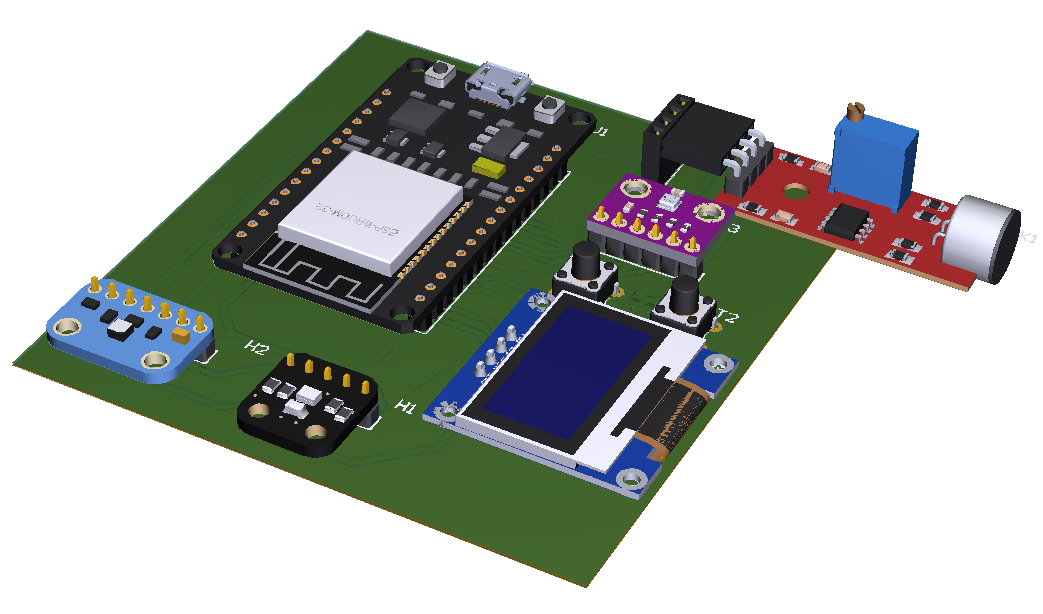
\includegraphics[width=10cm]{pcb}
\caption{Visão 3D da PCB}
\label{fig:img4}
\end{figure}

\section{Validação da Rede Mesh}

Visando validar a parte de comunicação sem fio utilizando BLE Mesh do ESP32 para o uso no projeto, uma rede simples com apenas 3 dispositivos foi desenvolvida. Dentre os dispositivos, 2 deles eram constituídos pelo microcontrolador escolhido conectados a de 3 LEDs cada um, e o terceiro um \textit{smartphone}. 

Arquitetura da rede de testes criada:

\begin{itemize}
	\item Nó com microcontrolador ESP32: 3 elementos, cada um com o \textit{OnOff Server Model} \cite{ble-mesh-models} implementado, visando controlar o ligamento e desligamento de um LED.
	\item \textit{Smartphone}: utilizando o aplicativo nRF Mesh \cite{nrf-app}, usado para provisionar os outros nós e controlar a rede \textit{mesh}.
\end{itemize}

O teste completo aqui descrito pode ser visto em \cite{teste-ble-mesh}.

A partir do aplicativo citado, os outros dois dispositivos foram provisionados, criando a rede \textit{mesh}. Depois, foram criados 3 grupos diferentes:

\begin{itemize}
	\item \textit{Red Lights}: grupo em que os \textit{models} que controlam os LEDs vermelhos nos nós foram inscritos;
	\item \textit{Green Lights}: grupo em que apenas um dos \textit{models} que controlam LEDs verdes foi incrito;
	\item \textit{Red and Blue}: grupo em que tanto os \textit{models} de LEDs vermelhas quanto os de LEDs azuis foram inscritos.
\end{itemize}

O funcionamento da rede pode ser validado quando mensagens de \textit{On} e \textit{Off} eram enviadas em cada grupo e apenas os LEDs que deveriam receber a mensagem do respectivo grupo era acionado ou desligado.

Foi possível visualizar o a criação e o funcionamento de uma rede BLE Mesh na plataforma escolhida, bastando apenas modificar a lógica e parâmetros necessários para que as mensagens contenham os dados coletados pelos sensores do projeto e sejam enviadas para os dispositivos desejados.



\end{document}